\documentclass[11pt,a4paper,oneside]{report}

\usepackage[spanish,es-noshorthands,es-tabla]{babel}
\usepackage[utf8]{inputenc}
\usepackage[T1]{fontenc}
\usepackage{lmodern}
\usepackage[margin=2.3cm,headheight=14pt]{geometry}
\usepackage{graphicx}
\usepackage[table]{xcolor}
\usepackage{booktabs}
\usepackage{tabularx}
\usepackage{enumitem}
\usepackage{titlesec}
\usepackage{fancyhdr}
\usepackage{float}
\usepackage{caption}
\usepackage[most]{tcolorbox}
\usepackage[hidelinks]{hyperref}

\graphicspath{{capturas/}}

% Paleta de Brasa Brava
\definecolor{brasa}{HTML}{F7941D}
\definecolor{carbon}{HTML}{1C1A17}
\definecolor{hueso}{HTML}{FAF4EA}
\definecolor{rojo}{HTML}{C1272D}

\hypersetup{colorlinks=true,linkcolor=carbon,urlcolor=brasa}
\setlist{itemsep=2pt,topsep=4pt}
\captionsetup{font=small,labelfont={bf,color=carbon}}

\titleformat{\chapter}[display]{\normalfont\bfseries\color{carbon}}{\large\color{brasa}\MakeUppercase{\chaptertitlename}~\thechapter}{4pt}{\Huge}
\titlespacing*{\chapter}{0pt}{0pt}{18pt}
\titleformat{\section}{\normalfont\Large\bfseries\color{carbon}}{\color{brasa}\thesection}{0.8em}{}
\titleformat{\subsection}{\normalfont\large\bfseries\color{carbon}}{\color{brasa}\thesubsection}{0.8em}{}

\pagestyle{fancy}
\fancyhf{}
\fancyhead[L]{\small\color{carbon!70}Brasa Brava · Manual de usuario}
\fancyhead[R]{\small\color{carbon!70}\leftmark}
\fancyfoot[C]{\small\thepage}
\renewcommand{\headrulewidth}{0.4pt}
\fancypagestyle{plain}{\fancyhf{}\fancyfoot[C]{\small\thepage}\renewcommand{\headrulewidth}{0pt}}

% Recuadros de ayuda
\newtcolorbox{consejo}{colback=hueso,colframe=brasa,boxrule=0.6pt,arc=2mm,left=8pt,right=8pt,top=6pt,bottom=6pt,fonttitle=\bfseries,title=Consejo}
\newtcolorbox{importante}{colback=rojo!5,colframe=rojo,boxrule=0.6pt,arc=2mm,left=8pt,right=8pt,top=6pt,bottom=6pt,fonttitle=\bfseries,title=Importante}

% Captura con su pie de figura
\newcommand{\captura}[3][0.92]{%
  \begin{figure}[H]
    \centering
    \includegraphics[width=#1\linewidth]{#2}
    \caption{#3}
  \end{figure}}

% Botones y textos de la pantalla
\newcommand{\boton}[1]{\textsf{\textbf{#1}}}
\newcommand{\pantalla}[1]{\textsf{#1}}

\begin{document}

\begin{titlepage}
  \pagecolor{carbon}\color{white}
  \centering
  \vspace*{3cm}
  {\color{brasa}\rule{\linewidth}{2pt}}\\[1.2cm]
  {\fontsize{44}{48}\selectfont\bfseries BRASA BRAVA}\\[0.4cm]
  {\Large Resto-Bar}\\[1.6cm]
  {\huge\bfseries Manual de usuario}\\[0.4cm]
  {\Large Sistema de gestión del restaurante}\\[1.2cm]
  {\color{brasa}\rule{\linewidth}{2pt}}
  \vfill
  {\large Caja, Familia, Reportes, Administración y Eliminación física}\\[0.3cm]
  {\large Versión de octubre de 2026}
\end{titlepage}
\nopagecolor\color{black}

\tableofcontents

\chapter{Introducción}

Este manual explica cómo usar el sistema de gestión de \textbf{Brasa Brava}, el que se usa en el local para tomar los pedidos de cada mesa, mandarlos a cocina, cobrar, revisar las ventas y mantener al día el menú, el inventario y el personal. Está pensado para leerse de corrido la primera vez y para consultarse después por partes: cada capítulo corresponde a una pantalla del menú.

\section{Qué hace el sistema}

\begin{tabla}{>{\titulos\bfseries}l X}
  \encabezado{Pantalla} & \encabezado{Para qué sirve} \\
  Página principal & Saludo, hora del local, resumen de caja y cocina del día y accesos rápidos \\
  Familia & Catálogo del local: productos, recetas, porciones que alcanzan con el stock y promociones \\
  Caja & Plano de mesas, armado del pedido, comanda para cocina, lo que ya salió, cobro y ticket \\
  Reportes & Ventas cobradas por fechas y por empleado, en PDF o por correo, y envíos automáticos \\
  Productos & Menú: precio, foto, categoría, disponibilidad y receta de cada producto \\
  Secciones & Ambientes del local y sus mesas con su capacidad \\
  Inventario & Insumos con su cantidad y su mínimo \\
  Categorías & Categorías y subcategorías del menú \\
  Promociones & Combos a precio fijo con sus fechas, días y horario \\
  Empleados & Personal, sus datos, su cargo y su acceso al sistema \\
  Cargos & Qué pantallas ve cada cargo \\
  Eliminación física & Borrado definitivo de lo dado de baja (solo el DIRECTORIO) \\
\end{tabla}

\section{Escritorio y web}

El sistema funciona de dos formas con las mismas pantallas y los mismos datos de cada local:

\begin{description}
  \item[Aplicación de escritorio (Windows).] Se abre como cualquier programa desde su ícono. Trae su propia base de datos, así que \textbf{no necesita internet} para vender. Es la que imprime directo en las ticketeras de cocina y de caja, sin abrir el diálogo de impresión. Al actualizarla no se pierde ningún dato.
  \item[Versión web.] Se abre en el navegador con la dirección que entregue el encargado del sistema. Imprime con el diálogo de impresión del navegador, donde se elige la ticketera.
\end{description}

Las pantallas se adaptan a computadora, tablet y celular. En pantallas angostas el menú se abre desde la barra naranja y las tablas se muestran como tarjetas (sección~\ref{sec:celular}).

\section{Quién ve qué}

Cada empleado tiene un \textbf{cargo}, y cada cargo tiene marcadas las pantallas que puede ver (sección~\ref{sec:cargos}). Si una pantalla no aparece en el menú es porque el cargo no la tiene. El \textbf{DIRECTORIO} es la cuenta del dueño: ve todo, cambia su propia contraseña, programa los envíos automáticos de reportes y es el único que puede hacer la eliminación física.

\begin{tabla}{>{\titulos\bfseries}l X}
  \encabezado{Cargo} & \encabezado{Pantallas con las que se instala el sistema} \\
  Administrador & Todas, menos la eliminación física \\
  Cajero & Página principal, Familia y Caja \\
  Mesero & Página principal, Familia y Caja \\
  Cocinero & Página principal y Familia \\
  DIRECTORIO & Todas, incluida la eliminación física \\
\end{tabla}

Los cargos se pueden cambiar y se pueden crear otros (por ejemplo, Bartender o Delivery) en \pantalla{Administración \guilsinglright{} Cargos}.

\section{Cómo leer este manual}

\begin{itemize}
  \item Los botones se escriben así: \boton{Enviar a cocina}.
  \item Las pantallas y menús, así: \pantalla{Administración \guilsinglright{} Productos}.
  \item Los campos de un formulario, en negrita: \campo{Correo de destino}.
  \item Los montos están en bolivianos (Bs) con coma decimal: Bs 85,00.
  \item Las fechas se muestran como día/mes/año y las horas en formato de 12 horas (AM/PM), siempre en la hora del local.
  \item Las capturas se tomaron con los datos de demostración del sistema; los nombres y montos de su local serán otros.
\end{itemize}

\begin{consejo}
Los campos obligatorios llevan un asterisco (*). Si falta algo o está mal escrito, el formulario no se guarda y el mensaje aparece en rojo debajo del campo, diciendo qué corregir.
\end{consejo}

\chapter{Ingreso al sistema}

\section{Iniciar sesión}

\captura{login}{Pantalla de inicio de sesión}

\begin{enumerate}
  \item Toque su foto en la fila de arriba, o escriba su \textbf{usuario} (por ejemplo, \texttt{a.romero}).
  \item Escriba su \textbf{contraseña}. El ojo del campo la muestra u oculta.
  \item Presione \boton{Ingresar}.
\end{enumerate}

Si la contraseña es incorrecta aparece un aviso rojo y el campo se vacía para volver a escribirla. Un empleado dado de baja no puede ingresar hasta que lo reactiven.

\section{Modo DIRECTORIO}

\captura{login-directorio}{Modo DIRECTORIO}

El dueño ingresa con el botón \boton{Modo directorio}: el usuario queda como \texttt{DIRECTORIO} y solo se escribe la contraseña de administración general. Para volver al ingreso normal se usa \boton{Modo empleado}.

El DIRECTORIO cambia su contraseña con el botón de la llave, junto a su nombre arriba a la derecha. Pide la contraseña actual y la nueva dos veces.

\section{Recuperar la contraseña}

\captura[0.8]{recuperar-contrasena}{Recuperar la contraseña}

\begin{enumerate}
  \item En el inicio de sesión toque \boton{¿Olvidaste tu contraseña?}.
  \item Escriba el correo de su cuenta y presione \boton{Enviar código}.
  \item Revise su correo: llega un código de 6 dígitos que vale 10 minutos. Escríbalo y presione \boton{Verificar}.
  \item Escriba la nueva contraseña dos veces (mínimo 8 caracteres, con letras y números) y presione \boton{Guardar contraseña}.
\end{enumerate}

\begin{importante}
El código admite 5 intentos. Si se equivoca más veces, pida un código nuevo. Si su cuenta está dada de baja, el sistema no envía el código: pida a administración que lo reactive.
\end{importante}

\section{Cerrar sesión}

Presione \boton{Cerrar sesión}, arriba a la derecha (en el celular está al final del menú). Hágalo siempre al terminar el turno, para que nadie registre pedidos a su nombre.

\chapter{Página principal y menú}
\label{cap:inicio}

\section{Página principal}

\captura{home}{Página principal}

Al ingresar se ve el saludo, la fecha y la hora del local. Quien tiene acceso a Caja ve además el \textbf{Resumen de hoy}, que se actualiza solo cada 30 segundos:

\begin{itemize}
  \item \textbf{Caja}: lo vendido y en cuántas ventas, lo cobrado en efectivo y por QR, y las mesas ocupadas con lo que falta cobrar.
  \item \textbf{Cocina}: los envíos en preparación, las unidades por preparar, los envíos listos para entregar y la espera más larga, con la mesa.
\end{itemize}

Más abajo están los \textbf{accesos rápidos} a las pantallas del cargo.

\section{Menú lateral}

El menú de la izquierda muestra solo las pantallas que su cargo puede ver. \pantalla{Administración} se despliega para mostrar sus pantallas. La pestaña redonda del borde contrae el menú para dejar solo los íconos, y el sistema recuerda cómo lo dejó.

\section{En celular y tablet}

\begin{figure}[H]
  \centering
  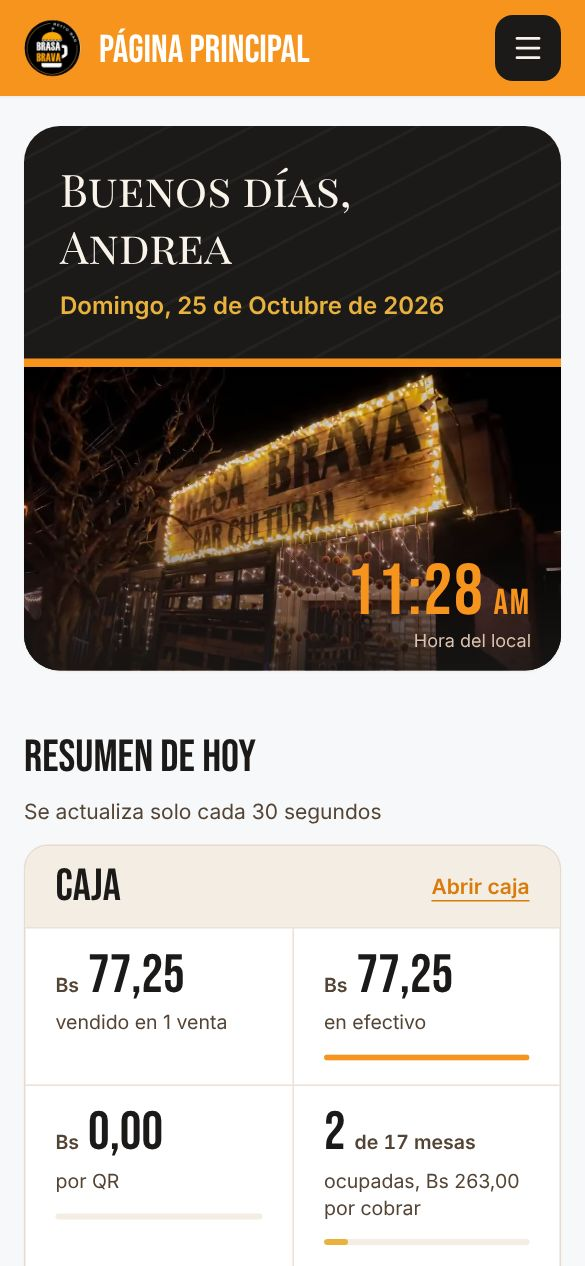
\includegraphics[width=0.3\linewidth]{celular-home}\hfill
  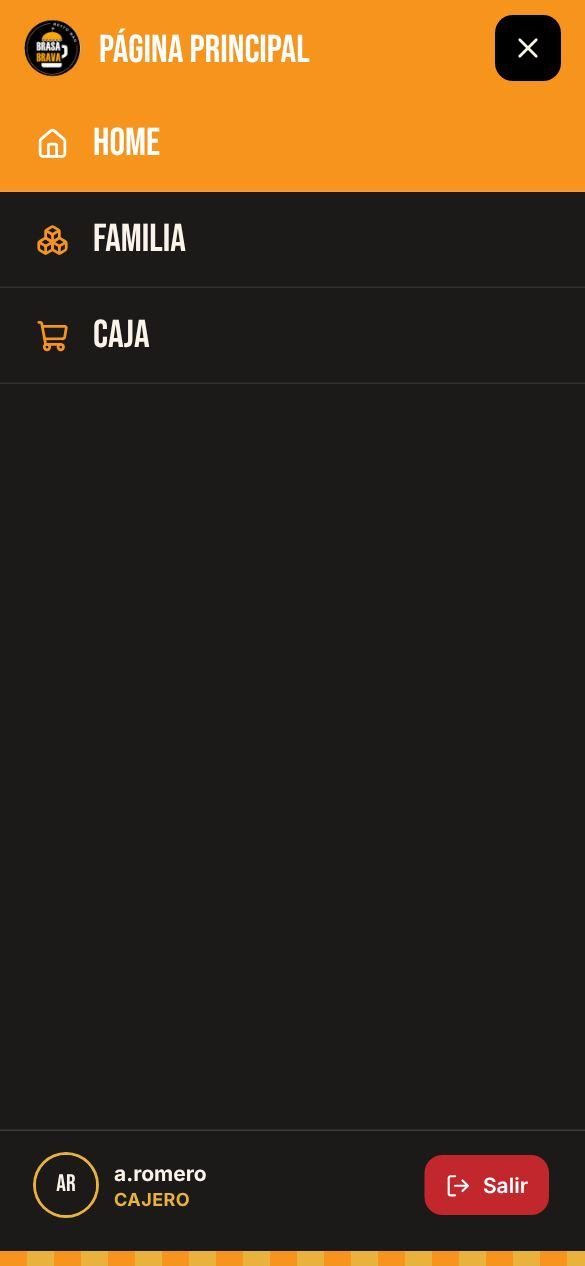
\includegraphics[width=0.3\linewidth]{celular-menu}\hfill
  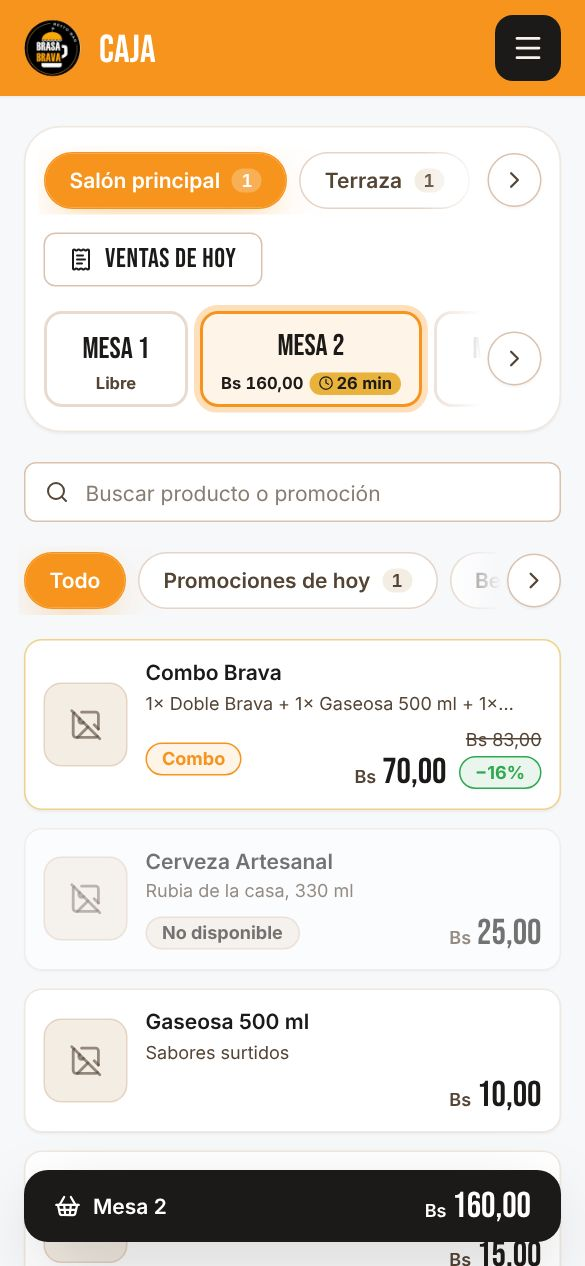
\includegraphics[width=0.3\linewidth]{celular-caja}
  \caption{Página principal, menú y Caja en el celular}
\end{figure}

En pantallas angostas el menú baja desde la barra naranja con el botón de la derecha y se cierra con la X, con la tecla Escape o al elegir una pantalla. Las tablas se muestran como tarjetas. En Caja, el pedido de la mesa se abre desde la barra inferior.

\chapter{Familia}

\pantalla{Familia} es el catálogo del local, para consultar sin cambiar nada. Sirve para que todo el personal sepa qué hay, cuánto cuesta y qué lleva cada producto.

\captura{familia}{Catálogo de productos}

\begin{itemize}
  \item Arriba se elige entre \boton{Productos} y \boton{Promociones}.
  \item La búsqueda encuentra productos aunque se escriban sin tildes.
  \item Los botones de categoría filtran el catálogo, y dentro de cada categoría se puede elegir una subcategoría.
  \item Las tarjetas avisan el stock: \textbf{Sin stock} si no alcanza para ninguna porción y \textbf{Agotado} si administración lo marcó como no disponible.
\end{itemize}

\captura[0.8]{familia-detalle}{Detalle de un producto con su receta}

Al tocar un producto se ve su precio, su descripción y su \textbf{receta}: cuánto lleva de cada insumo por porción y para cuántas porciones alcanza el stock de cada uno. Si no alcanza para ninguna, el aviso dice qué insumo falta; el producto se puede vender igual, pero conviene avisar a cocina.

En \boton{Promociones} cada combo muestra qué productos incluye, cuánto se ahorra y cuándo aplica (fechas, días y horario).

\chapter{Caja}

\pantalla{Caja} reúne en una sola pantalla todo el recorrido de una mesa: elegirla, armar el pedido, mandarlo a cocina, marcar lo que sale y cobrar. Cocina no usa el sistema: recibe la \textbf{comanda impresa}, y el cajero marca en Caja lo que ya salió.

\captura{caja}{Caja sin mesa elegida}

La pantalla tiene tres partes:

\begin{description}
  \item[Arriba, las mesas.] Las secciones del local (Salón principal, Terraza, Barra…) con cuántas mesas ocupadas tiene cada una, y las mesas de la sección elegida. Una mesa libre dice \textbf{Libre}; una ocupada muestra lo que lleva consumido y hace cuánto espera lo que falta de cocina. La espera se pinta de amarillo desde los 15 minutos y de rojo desde los 30.
  \item[A la izquierda, el pedido] de la mesa elegida.
  \item[A la derecha, el menú del día] con buscador y categorías. \boton{Promociones de hoy} muestra solo los combos que valen en este momento.
\end{description}

\section{Tomar un pedido}

\begin{enumerate}
  \item Toque la mesa en la barra de arriba. Si no eligió mesa, el menú le recuerda hacerlo primero.
  \item Toque un producto o una promoción del menú. Se abre su ventana:
\end{enumerate}

\captura[0.75]{caja-agregar-producto}{Agregar un producto: cantidad, consumo e ingredientes}

\begin{itemize}
  \item \textbf{Cantidad}: con $-$ y $+$.
  \item \textbf{Consumo}: \boton{Local} si se sirve en la mesa o \boton{Para llevar}.
  \item \textbf{Quitar ingredientes}: toque los que el cliente no quiere; quedan tachados en rojo. En un combo se eligen por cada producto del combo.
  \item Presione \boton{Agregar al pedido}.
\end{itemize}

\begin{consejo}
Si dos hamburguesas llevan cambios distintos (una sin tomate y otra completa), agréguelas por separado. Cuando se agrega algo igual a una línea que ya está, el sistema las junta y suma la cantidad.
\end{consejo}

\captura{caja-pedido-nuevo}{Pedido por registrar}

Lo agregado aparece en \textbf{Por registrar}, en columnas: \textbf{Cant.}, \textbf{Producto}, \textbf{Consumo} y \textbf{Bs}. Lo quitado se lee en rojo debajo del nombre. Cada línea se puede ajustar con $-$ y $+$, cambiar con el lápiz o quitar con el tacho.

En el menú, los productos con poco stock dicen \textbf{Quedan N} o \textbf{Sin stock}, pero se pueden vender igual; los marcados como agotados no se pueden elegir.

\section{Enviar a cocina}

Presione \boton{Enviar a cocina}. Si la mesa estaba libre se abre la venta con su número de pedido; si ya estaba ocupada, lo nuevo se suma como un \textbf{envío} más. El stock de los insumos se descuenta según la receta.

\captura[0.75]{caja-comanda}{Comanda de cocina del envío}

La \textbf{comanda} lleva solo lo nuevo de ese envío, con la mesa, el número de pedido, el cajero que lo registró, lo quitado (\textit{sin: tomate}) y el consumo de cada línea (\textbf{L} local, \textbf{LL} para llevar). No lleva precios. Desde el segundo envío dice \textbf{MODIFICADO POR} y el nombre de quien lo registró.

\begin{itemize}
  \item En la \textbf{aplicación de escritorio} con impresora de cocina elegida, la comanda se imprime sola.
  \item En el navegador se muestra la vista previa: presione \boton{Imprimir}.
\end{itemize}

Si un insumo no alcanzó, aparece el aviso \textit{Revise el inventario}: el pedido se envió igual y ese insumo quedó en cero.

\begin{importante}
Si cambia de mesa con productos todavía sin enviar, el sistema pregunta antes de descartarlos. Envíelos a cocina primero si no quiere perderlos.
\end{importante}

\section{Lo ya registrado en una mesa}

\captura{caja-mesa-ocupada}{Mesa ocupada con su pedido registrado}

Al elegir una mesa ocupada se ve quién la abrió, desde qué hora y cuánto espera. En \textbf{Registrado} aparece cada envío con su hora y \textbf{quién lo registró} (por ejemplo, \textit{Envío 2 · 8:31 PM · Registró: admin}), y debajo de cada producto cuántas unidades ya salieron de cocina. El botón de impresora de cada envío vuelve a imprimir su comanda; la comanda se puede reimprimir las veces que haga falta.

El pedido ya no lleva mesero: solo queda registrado el empleado que tomó cada envío.

\section{Marcar lo que sale de cocina}

\captura{caja-marcar-listos}{Marcar listos}

Cuando cocina entrega, presione \boton{Marcar listos}. La ventana tiene tres columnas:

\begin{description}
  \item[Local] y \textbf{Para llevar}: cada producto pendiente con $-$ y $+$ para marcar las unidades que salieron, y el botón verde para marcarlo completo.
  \item[Faltan]: lo que todavía no salió. Cuando no falta nada dice que ya se puede cobrar.
\end{description}

\boton{Todo listo} marca de una vez todo lo pendiente de la mesa.

\section{Cobrar}

\boton{Cobrar} se habilita recién cuando no falta nada de cocina.

\captura{caja-cobro}{Cobro de la mesa}

\begin{enumerate}
  \item Elija la forma de pago: \boton{Efectivo}, \boton{QR} o \boton{Mixto} (una parte en efectivo y el resto por QR).
  \item En efectivo, escriba lo que entregó el cliente o use los montos rápidos (\boton{Exacto}, Bs 90, Bs 100…). El sistema calcula el cambio. Si el monto no alcanza, avisa cuánto falta. Si paga exacto puede dejarlo vacío.
  \item Presione \boton{Cobrar Bs …}.
\end{enumerate}

A la izquierda se ve la vista previa del ticket. El enlace \boton{Página de impuestos} abre la página para emitir la factura.

\captura[0.75]{caja-ticket}{Ticket de venta}

Al cobrar, la mesa queda libre y se imprime el \textbf{ticket de venta}, que junta las líneas iguales y lleva el total, la forma de pago, lo recibido y el cambio.

\section{Límite de impresiones del ticket}

El ticket de una venta se puede imprimir \textbf{3 veces} libremente (contando la del cobro). Desde la cuarta, el sistema pide el usuario y la contraseña de un empleado con acceso a Caja, y deja registrado quién la autorizó.

\captura[0.75]{caja-autorizar-reimpresion}{Autorización para la cuarta impresión}

\section{Ventas de hoy}

\captura[0.8]{caja-ventas-hoy}{Ventas de hoy}

\boton{Ventas de hoy}, arriba a la derecha de las mesas, muestra las ventas cobradas del día con sus totales (ventas, total, efectivo y QR). Cada venta tiene su botón para reimprimir el ticket, con el mismo límite de impresiones. Quien tiene acceso a Administración puede cambiar aquí el enlace de la página de impuestos.

\section{Impresoras (aplicación de escritorio)}

En la aplicación de escritorio aparece el botón \boton{Impresoras} junto a \boton{Ventas de hoy}. Ahí se elige la impresora de \textbf{cocina} (comandas) y la de \textbf{caja} (tickets) de esa computadora, y \boton{Imprimir prueba} saca una hoja para comprobarla. Si una impresión directa falla, el sistema avisa y ofrece \boton{Imprimir con diálogo}.

\chapter{Reportes de ventas}

\pantalla{Reportes} muestra las ventas \textbf{cobradas}, según la hora en que se cobraron. Al abrirla trae el resumen de hoy.

\section{Elegir qué ver}

\captura{reportes-resumen}{Resumen de ventas}

\begin{enumerate}
  \item Elija el tipo: \boton{Resumen de ventas} o \boton{Ventas detalladas}.
  \item Elija las fechas \textbf{Desde} y \textbf{Hasta} con el calendario, o use los atajos \boton{Hoy}, \boton{Ayer}, \boton{Esta semana} y \boton{Este mes}.
  \item Si quiere, elija un \textbf{Empleado}: trae las ventas que esa persona registró, a las que agregó un envío o que cobró. También se puede elegir el DIRECTORIO. Los empleados dados de baja aparecen marcados como \textit{de baja}.
  \item Presione \boton{Generar}.
\end{enumerate}

Arriba de la tabla están los totales del período: cantidad de ventas, total, efectivo, QR y ticket promedio.

\begin{description}
  \item[Resumen de ventas] tiene una fila por día con sus ventas, efectivo, QR y total.
  \item[Ventas detalladas] tiene una fila por venta: número, hora de cobro, mesa, quién la abrió y quién la cobró, y los montos.
\end{description}

\captura{reportes-detalladas}{Ventas detalladas}

\section{Detalle de una venta}

\captura{reportes-venta}{Detalle de una venta}

El ojo de cada fila abre la venta completa:

\begin{itemize}
  \item Cada \textbf{envío} con su hora y quién lo registró, en una tabla con \textbf{Cant.}, \textbf{Producto}, \textbf{Consumo} (Local o Para llevar) y \textbf{Subtotal}. Lo quitado se lee en rojo debajo del producto.
  \item El \textbf{cobro}: efectivo, QR, total, recibido, cambio, quién cobró y cuándo.
  \item Cuántas veces se imprimió el ticket.
\end{itemize}

\boton{Reimprimir ticket} vuelve a imprimirlo, con el mismo límite de impresiones de Caja (solo quien tiene acceso a Caja).

\section{Descargar o enviar por correo}

\begin{itemize}
  \item \boton{Descargar PDF} guarda el reporte que se está viendo. El PDF de ventas detalladas trae cada venta con su tabla de productos.
  \item Para mandarlo, escriba un correo en \textbf{Enviar a este correo} y presione \boton{Enviar por correo}: llega con el PDF adjunto.
\end{itemize}

\begin{importante}
Para que los correos salgan de verdad, la computadora debe tener configurada la clave del servicio de correo (Brevo), la misma que usa la recuperación de contraseñas. Pídasela al encargado del sistema.
\end{importante}

\section{Envíos programados (solo el DIRECTORIO)}

El DIRECTORIO puede hacer que el reporte llegue solo por correo ciertos días a cierta hora.

\captura[0.8]{reportes-nuevo-envio}{Nuevo envío programado}

\begin{enumerate}
  \item Presione \boton{Envíos programados} y luego \boton{Nuevo envío}.
  \item Escriba el \textbf{correo de destino}, elija el \textbf{reporte}, marque los \textbf{días de la semana} y la \textbf{hora}.
  \item Presione \boton{Guardar}.
\end{enumerate}

\captura[0.8]{reportes-programados}{Lista de envíos programados}

En la lista, cada envío muestra cuándo salió el último y cuándo sale el próximo. Con sus botones se puede:

\begin{itemize}
  \item \textbf{Pausar} o reanudar con el interruptor.
  \item \textbf{Enviar ahora}, sin esperar el día y la hora.
  \item \textbf{Modificar} con el lápiz o \textbf{borrar} con el tacho.
\end{itemize}

Cómo funciona:

\begin{itemize}
  \item Cada envío trae las ventas \textbf{desde el envío anterior} hasta ese momento.
  \item Si la computadora estaba apagada a esa hora, el reporte sale apenas se enciende el sistema y en la lista figura como \textit{Enviado al encender}.
  \item Si el correo falla, el sistema lo vuelve a intentar solo a los 15 minutos.
\end{itemize}

\chapter{Administración}

Las pantallas de \pantalla{Administración} mantienen al día el menú, el local y el personal. Todas funcionan igual.

\section{Cómo funcionan las pantallas de gestión}

\begin{itemize}
  \item \textbf{Buscar}: el buscador filtra mientras se escribe.
  \item \textbf{Filtros}: los selectores de arriba (estado, categoría, cargo…). \boton{Limpiar filtros} los quita.
  \item \textbf{Ordenar}: toque el encabezado de una columna; otra vez invierte el orden.
  \item \textbf{Filas por página} y las flechas de abajo para pasar de página.
  \item \textbf{Registrar}: el botón naranja del final (\textit{¿Desea registrar…?}).
  \item \textbf{Acciones} de cada fila: el lápiz modifica; el círculo tachado \textbf{da de baja}; la flecha \textbf{reactiva}.
\end{itemize}

Los filtros y el orden quedan en la dirección de la página, así que al volver atrás se conservan.

\begin{consejo}
\textbf{Dar de baja no borra nada}: el registro deja de usarse pero se conserva con su historial (las ventas viejas siguen mostrando ese producto o ese empleado). Lo dado de baja aparece tachado y se puede reactivar. Para borrarlo para siempre está la eliminación física (capítulo~\ref{cap:eliminacion}).
\end{consejo}

\section{Productos}

\captura{productos}{Gestión de productos}

Cada producto tiene nombre, precio, foto, categoría y subcategoría, descripción y su receta. La columna \textbf{Disponible} es un interruptor: apagado, el producto figura como \textbf{Agotado} y no se puede vender en Caja hasta encenderlo de nuevo. La columna \textbf{Receta} dice para cuántas porciones alcanza el stock, o \textit{Sin insumos} si falta alguno.

\captura[0.7]{productos-registrar}{Registrar un producto}

Para registrar, elija primero la categoría y después la subcategoría. El precio se escribe con coma decimal.

\subsection{Receta}

\captura[0.7]{productos-receta}{Receta de un producto}

El botón del gorro de cocinero abre la \textbf{receta}: los insumos que lleva una porción y cuánto de cada uno. Caja descuenta esas cantidades del inventario en cada venta. Debajo se ve para cuántas porciones alcanza el stock actual.

\section{Secciones y mesas}

\captura{secciones}{Gestión de secciones}

Las secciones son los ambientes del local. Cada una tiene sus mesas con su capacidad.

\captura[0.7]{secciones-registrar}{Registrar una sección con sus mesas}

\boton{Agregar mesa} suma una mesa numerada automáticamente; la capacidad se ajusta con sus botones. Una mesa que se quita deja de aparecer en Caja, pero sus ventas anteriores se conservan.

\section{Inventario}

\captura{inventario}{Inventario de insumos}

Cada insumo tiene su unidad (kilogramos, litros o unidades), la cantidad actual y el \textbf{mínimo}. La cantidad se pinta según el nivel: en rojo cuando no queda nada y en naranja cuando llegó al mínimo o está por debajo.

Para corregir la cantidad después de contar el depósito, modifique el insumo y escriba la cantidad real: queda registrado como un ajuste.

\section{Categorías}

\captura{categorias}{Gestión de categorías}

\captura[0.7]{categorias-registrar}{Registrar una categoría}

Cada categoría del menú tiene foto, descripción y sus \textbf{subcategorías} (por ejemplo, Hamburguesas → Clásicas, Especiales, Doble Carne). Las subcategorías se agregan, renombran o quitan en el mismo formulario. Una categoría dada de baja deja de mostrarse en el menú de Caja.

\section{Promociones}

\captura{promociones}{Gestión de promociones}

Las promociones son \textbf{combos a precio fijo}: varios productos con sus cantidades por un precio menor al que costarían por separado.

\captura[0.7]{promociones-registrar}{Registrar una promoción}

\begin{itemize}
  \item Agregue los productos con \boton{Agregar producto} y su cantidad. El sistema muestra en vivo el precio por separado y el ahorro.
  \item Elija la fecha \textbf{Desde} y, si quiere, \textbf{Hasta} (vacía, no vence).
  \item Marque los \textbf{días} en que vale (obligatorio) y, si quiere, un \textbf{horario} (por ejemplo, 6:00 PM a 9:00 PM).
\end{itemize}

La columna \textbf{Vigencia} dice su estado: \textit{Vigente ahora}, \textit{Hoy no aplica}, \textit{Programada}, \textit{Vencida} o \textit{Inactiva}. Solo las vigentes en ese momento aparecen en \boton{Promociones de hoy} de Caja.

\section{Empleados}

\captura{empleados}{Gestión de empleados}

\captura[0.7]{empleados-registrar}{Registrar un empleado}

Para registrar un empleado se cargan sus datos personales (nombre, apellido, CI, teléfono), su foto, su cargo, su correo y su contraseña inicial. El \textbf{usuario} se sugiere con el nombre y el apellido, y se puede cambiar. El correo es el que usará para recuperar la contraseña. Al modificar, la contraseña se deja vacía para mantener la actual.

Un empleado dado de baja no puede ingresar al sistema, pero sus ventas se conservan.

\section{Cargos}
\label{sec:cargos}

\captura{cargos}{Gestión de cargos}

Cada cargo tiene marcadas las pantallas que ve quien lo tenga.

\captura[0.75]{cargos-modificar}{Pantallas de un cargo}

\begin{itemize}
  \item La página principal la tienen todos.
  \item Las pantallas están agrupadas en \textbf{Operación del local} y \textbf{Administración}; \boton{Marcar todas} marca un grupo entero.
  \item Antes de guardar, el formulario avisa a cuántos empleados afecta el cambio; lo verán la próxima vez que inicien sesión.
  \item Un cargo no se puede dar de baja mientras tenga empleados activos.
  \item La eliminación física no se puede dar a ningún cargo: es solo del DIRECTORIO.
\end{itemize}

\chapter{Eliminación física}
\label{cap:eliminacion}

\begin{importante}
Lo que se elimina aquí \textbf{se borra para siempre} junto con todo lo que depende de ello, y no se puede recuperar. Solo el DIRECTORIO entra a esta pantalla, y ningún cargo puede recibir este permiso.
\end{importante}

\section{Qué se puede eliminar}

\captura{eliminacion}{Eliminación física}

Solo se puede elegir lo que \textbf{ya está dado de baja} y las \textbf{ventas ya cobradas}. Hay una pestaña por tipo: empleados, cargos, secciones y mesas, productos, categorías, insumos, promociones y ventas. Cada pestaña dice cuántos registros tiene marcados.

\begin{enumerate}
  \item Entre a \pantalla{Administración → Eliminación física}.
  \item En cada pestaña, toque las filas que quiere borrar. \boton{Marcar todos} y \boton{Quitar marcas} ayudan con muchas filas. En \textbf{Ventas} primero se eligen las fechas.
  \item Se puede marcar en varias pestañas y borrar todo junto con \boton{Eliminar N marcados}.
\end{enumerate}

\section{Qué arrastra cada cosa (en cascada)}

Al eliminar algo se borra también todo lo que depende de eso. Cada fila avisa lo que arrastra, por ejemplo \textit{2 ventas se borran también}.

\begin{table}[H]
  \centering
  \caption{Lo que se borra junto con cada registro}
  \rowcolors{2}{hueso}{white}
  \begin{tabularx}{\linewidth}{lX}
    \toprule
    \textbf{Si elimina…} & \textbf{También se borra} \\
    \midrule
    Un cargo & Sus empleados \\
    Un empleado & Las ventas que abrió, a las que agregó un envío o que cobró \\
    Una sección & Sus mesas y las ventas de esas mesas \\
    Una categoría & Sus subcategorías y sus productos \\
    Un producto & Su receta, las promociones que lo incluyen y las ventas donde aparece \\
    Una promoción & Las ventas donde se vendió \\
    Un insumo & Su lugar en las recetas, sus movimientos y las ventas donde se quitó \\
    Una venta & Sus productos, envíos, pagos e impresiones del ticket \\
    \bottomrule
  \end{tabularx}
\end{table}

\section{Confirmar}

\captura[0.8]{eliminacion-confirmar}{Confirmación de la eliminación}

Antes de borrar, el sistema muestra \textbf{todo lo que se va}, incluido lo que arrastra. Para seguir hay que escribir la palabra \texttt{ELIMINAR} y presionar \boton{Sí, eliminar}.

Si algo de lo elegido sigue activo, o si arrastra una mesa con un pedido abierto, el sistema dice qué lo impide y no deja seguir: dé de baja ese registro o cobre el pedido antes.

\begin{consejo}
Antes de una eliminación grande, descargue el PDF de Reportes del período que se va a borrar: las ventas eliminadas dejan de aparecer en los reportes.
\end{consejo}

\chapter{Preguntas frecuentes}

\paragraph{No puedo ingresar} Revise que el usuario esté bien escrito (por ejemplo, \texttt{a.romero}, con punto) o toque su foto. Si olvidó la contraseña, use \boton{¿Olvidaste tu contraseña?}. Si el sistema dice que su cuenta está dada de baja, pida a administración que la reactive.

\paragraph{No me llega el código de recuperación} Revise la carpeta de correo no deseado y que el correo sea el registrado en su cuenta. El código vale 10 minutos; si venció, pida otro. Si nunca llegan correos, falta configurar el servicio de correo en el sistema.

\paragraph{No veo una pantalla del menú} Su cargo no la tiene marcada. Pida a quien administra los cargos que la agregue; la verá la próxima vez que inicie sesión.

\paragraph{El sistema me sacó y pide ingresar de nuevo} La sesión dura un turno (8 horas). Ingrese otra vez: vuelve a la pantalla en la que estaba.

\paragraph{El botón Cobrar está gris} Todavía falta algo de cocina. Abra \boton{Marcar listos} y marque lo que ya salió; cuando la columna \textbf{Faltan} quede vacía, se habilita el cobro.

\paragraph{Un producto no se puede elegir en Caja} Está marcado como agotado. Quien tenga acceso a Productos debe encender su interruptor \textbf{Disponible}. Si directamente no aparece, está dado de baja o su categoría lo está.

\paragraph{Una promoción no aparece en Caja} Solo aparecen las vigentes en ese momento. Revise en \pantalla{Promociones} sus fechas, días y horario: la columna Vigencia dice por qué no aplica.

\paragraph{Apareció «Revise el inventario» al enviar un pedido} Algún insumo de la receta no alcanzó: el pedido se envió igual y ese insumo quedó en cero. Cargue la cantidad real en \pantalla{Inventario}.

\paragraph{Me equivoqué en un pedido ya enviado} Lo enviado a cocina no se borra desde Caja. Avise a cocina y, si hace falta, registre lo correcto en un nuevo envío.

\paragraph{El ticket pide usuario y contraseña} Ya se imprimió 3 veces. Un empleado con acceso a Caja debe autorizar la nueva impresión; queda registrado quién lo hizo.

\paragraph{La comanda o el ticket no salen por la impresora} En la aplicación de escritorio, revise en \boton{Impresoras} que estén elegidas la de cocina y la de caja, y pruebe con \boton{Imprimir prueba}. Revise que la impresora esté encendida y con papel. Si la impresión directa falla, use \boton{Imprimir con diálogo}. En el navegador, elija la ticketera en el diálogo de impresión.

\paragraph{El reporte no llega por correo} Revise que el correo esté bien escrito y la carpeta de correo no deseado. Si los correos nunca salen, falta configurar la clave del servicio de correo en esa computadora. En los envíos programados que fallaron, el sistema vuelve a intentar solo a los 15 minutos.

\paragraph{La computadora estaba apagada a la hora de un envío programado} El reporte sale apenas se enciende el sistema, con las ventas desde el envío anterior, y en la lista figura como \textit{Enviado al encender}.

\paragraph{No puedo dar de baja una sección o un cargo} Una sección con mesas ocupadas no se da de baja hasta cobrarlas. Un cargo que tienen empleados activos tampoco: primero cámbieles el cargo.

\paragraph{Borré algo en la eliminación física} No se puede deshacer. Por eso la pantalla muestra antes todo lo que se va y pide escribir \texttt{ELIMINAR}. Si solo quería que algo dejara de usarse, alcanza con darlo de baja.


\end{document}
